\subsection{Layer restoring performance -- aware deduplication}
\label{sec:design_operations}

%\paragraph{Workflow}
%
%The proposed Docker registry API is very similar to the original API.
%%Interactions with the Docker client is unchanged: 
%A user simply pushes and pulls images to and from the registry. 
In the following, we describe our \sysname~layer restoring performance --aware deduplication
 (i.e., \sysname~\dedupname) design. 
%explain Docker operations integration with \sysname.

%\sysname~ is composed of five main components(see Figure~\ref{onshareddir}):
%a modified Docker client,
%layer buffer,
%file cache,
%registries,
%backend storage system that implements deduplication.
%The modified Docker client sends put or pull layer/manifest requests.
%After it sends the pull layer requests.
%it receives multiple partial layers and decompresses them together as a whole uncompressed layer, then verifies the
%integrity of the uncompress layer by calculating the digest of the uncompress layer.
%Layer buffer is used to buffer all the put layer requests and 
%cache prefetched layers for later use.

\subsubsection{When to deduplicate layers?}

\begin{figure*}[t]
\centering
			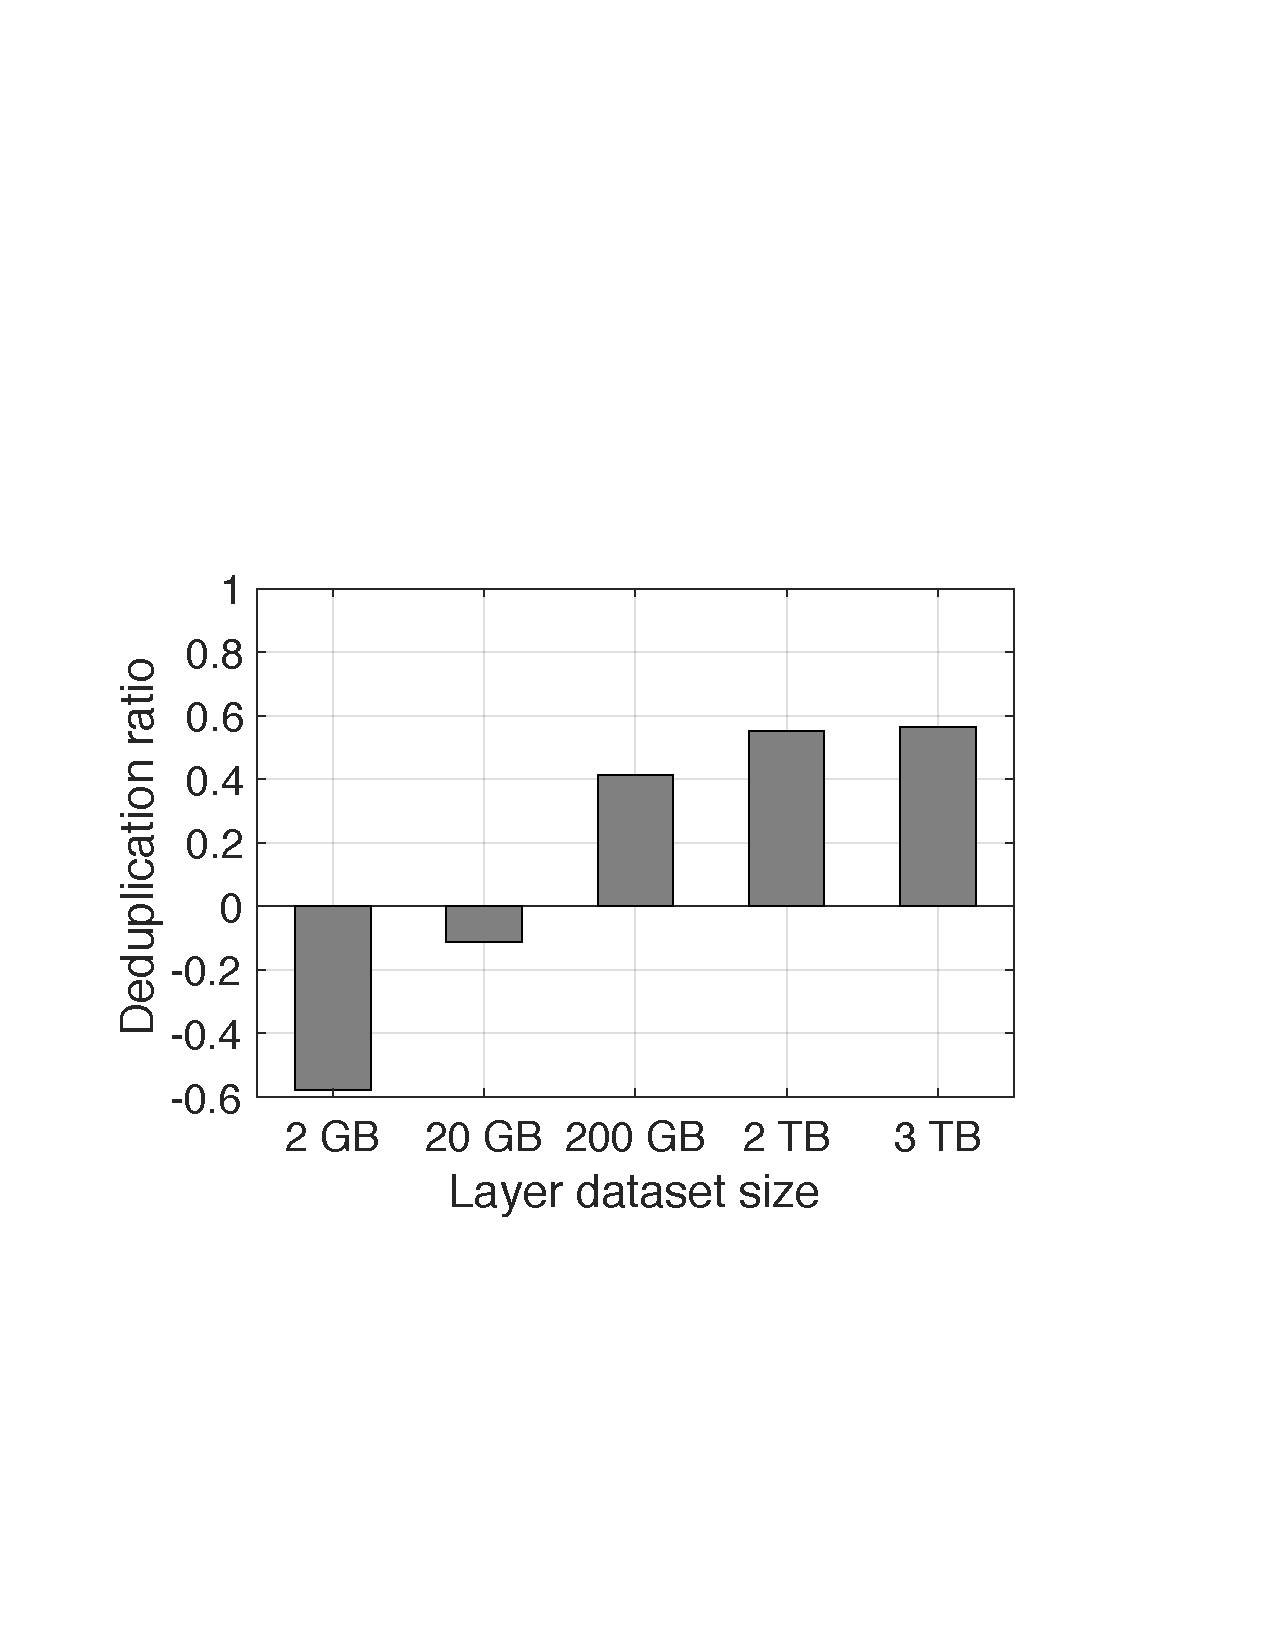
\includegraphics[width=0.2\textwidth]{graphs/dedup_vs_compression.pdf}
			\caption{Efficiency of deduplication over compression}
		%	\vspace{-3pt}
			\label{fig:cacheefficiency}

\end{figure*}

%\begin{figure}[t]
%	\centering
%	\begin{minipage}{0.26\textwidth}
%		\centering
%		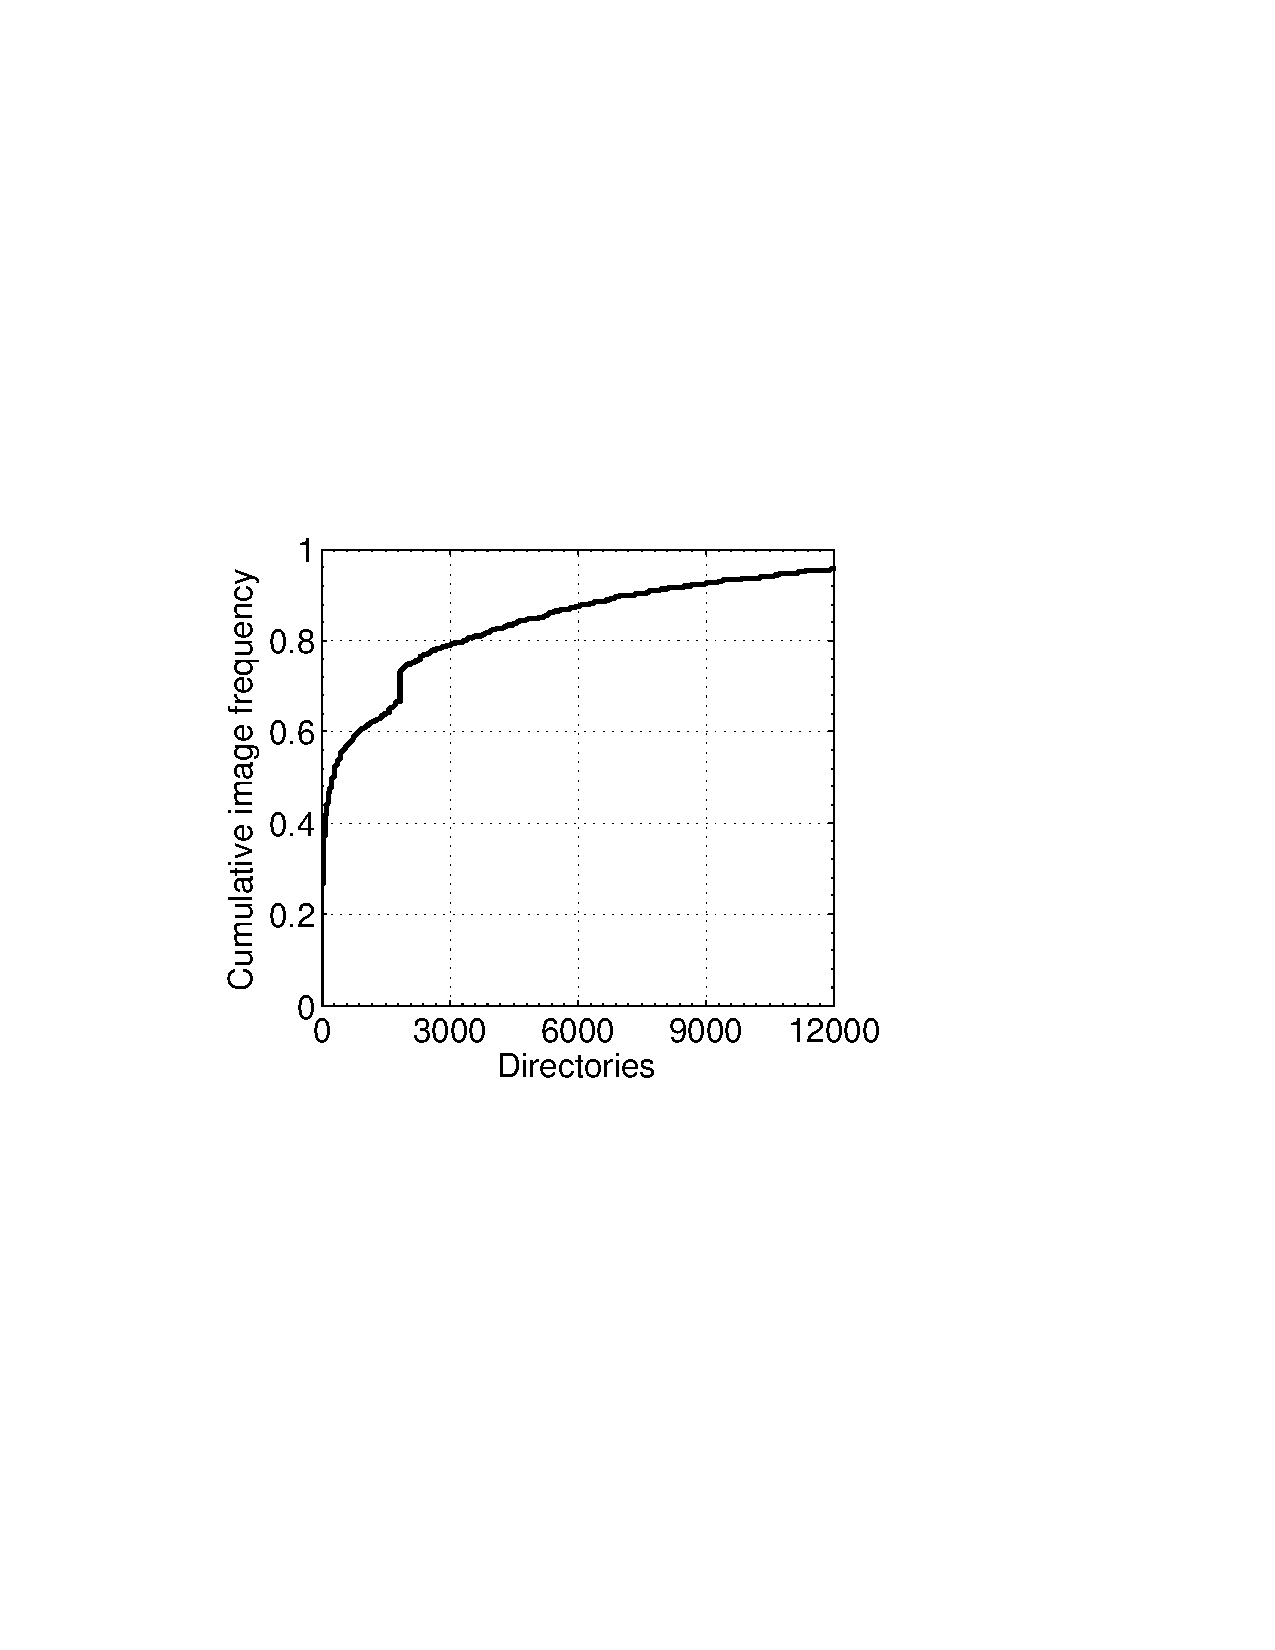
\includegraphics[width=1\textwidth]{graphs/dir.pdf}
%		\caption{CDF of images by\newline directories}
%		\label{fig-dir}
%	\end{minipage}%
%	\begin{minipage}{0.24\textwidth}
%		\centering
%		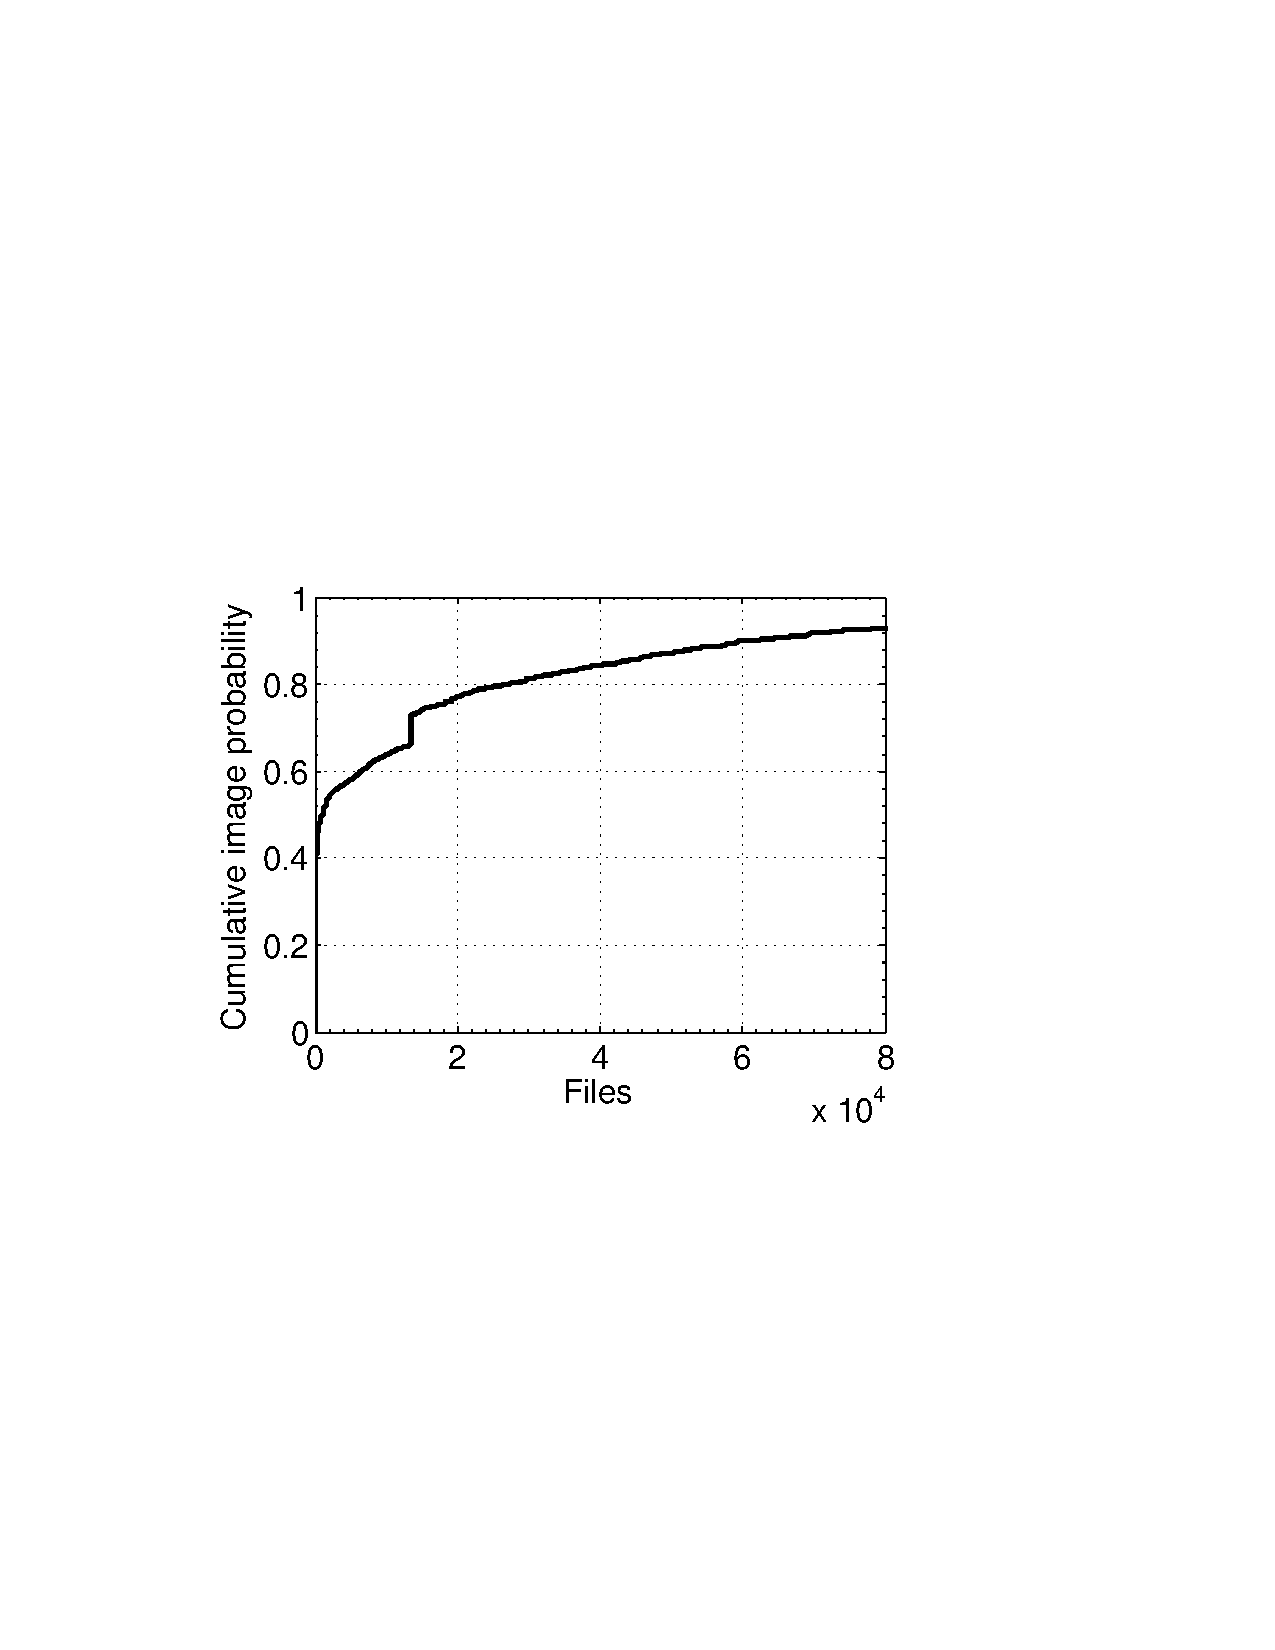
\includegraphics[width=1\textwidth]{graphs/file.pdf}
%		\caption{CDF of images by files}
%		\label{fig-file}
%	\end{minipage}
%\end{figure}

%\begin{figure}[htbp] 
%	\begin{minipage}{0.5\linewidth} 
%		\centering 
%		\includegraphics{circle} 
%		\caption{A Circle} 
%		\label{fig:circle} 
%	\end{minipage}% 
%	\begin{minipage}{0.5\linewidth} 
%		\centering 
%		\includegraphics{rectangle} 
%		\caption{A Rectangle} 
%		\label{fig:rectangle} 
%	\end{minipage} 
%\end{figure}

Consider that deduplication incurs performance overhead and current registry already stores layers in compressed format to save space and network transfer overhead, 
 we first analyze the space efficiency of a registry that performs decompress and file-level deduplication compared to 
 a registry that naively stores compressed layers.

In Figure~\ref{fig:cacheefficiency}, the x-axis values correspond to the sizes of $5$ random samples drawn from the whole dataset detailed in xxx and the size of the dataset in terms of capacity and layer count.
For a traditional registry, the compressed layer tarballs will be kept as is.
While a registry with file-level deduplication will store \emph{deduplicated} layers (i.e., unique files). 
The y-axis shows how much space a registry with file-level deduplication can save compared to naively storing compressed layer tarballs.
For the first two samples of the dataset, with size less than $20$~GB, 
there is no benefit to \emph{deduplicate} layers 
because the deduplication ratio is very low.
However, when the dataset size is $3$~TB, we can save $56\%$ more space.
The space saved by applying decompression and file-level deduplication increases almost linearly with the size of the layer dataset.
This verifies the benefit of deduplicate layers when the dataset is large, which should be carefully selected to realize significant space savings.

\subsubsection{Layer deduplication}

After receiving a \texttt{push} layer request, \sysname~\dedupname~will store the layer as it is and return a response back to client. 
\dedupname~initiates layer deduplication process only if layer deduplication will achieve significant space savings and the process won't impact foreground requests. 
Sepcially, layer deduplication process is triggered when
the layer dataset $S$ is greater than a predefined threshold $\delta_{s}$ and the registry traffic $RPS$ ( i.e., requests per second) is lower than $\delta_{RPS}$. Thus, layer deduplication process runs periodically.
The process always stars with the cold layers that haven't been
access for a long time.
  
The deduplication process has tree major steps: layer decompression, file-level deduplication,
and unique file distribution. 
The first two steps are necessary for removing file duplicates from compressed layer tarballs.
The last step unique file distribution is to balance the layer restoring load among registries so that 
layer restoring process will achieve an optimal parallelism for each layer (detailed in xxx) and 
accelerate layer restoring process. 
After layer deduplication, unique files are evenly distributed across multiple registry servers. 
We define all the per-server files belonging to a layer as a {\em slice}. 
A server stores slices for many layers, and a layer is composed of slices stored on multiple servers, which allows restoring a layer in parallel. 

Similar with traditional file-level deduplication, \dedupname~maintains file fingerprint indexes to address the corresponding files in the storage system. 
Similar with traditional registry, \dedupname~maintains layer fingerprint indexes to address the corresponding layers stored in the system.
Besides, \dedupname~creates a list of slice recipes identified by layer digest for each layer that is deduplicated. 
Slice recipe contains partial of the layer tarball's directory tree structure, file digests, and file metadata information (such as, permission and attributes), which are needed for restoring a slice for the layer. Note that, layer deduplication process only deduplicate regular files.
Figure~\ref{xxx} shows an example of layer fingerprint indexes, file fingerprint indexes, and slice recipe.
Fingerprint indexes, layer recipes, and \sysname~manifest are stored on distributed NoSQL databases
for reliability, consistency, and fast accesses.

The deduplication process is detailed as follows:
\begin{compactenumerate}
	\item  check the layer fingerprint in the \emph{layer fingerprint index} to ensure 
	an identical layer is not already stored.
	\item decompress and unpack the unique layer into files;
	\item compute a \emph{fingerprint} for every file in the layer;
	\item check every file's fingerprint in the \emph{file fingerprint index} to
	ensure an identical file is not already stored;
	\item distribute the newly added unique files to the registry cluster by using round-robin, and;
	 \item calculate the slice digests based on unique file redistribution, and
	 update the manifest by using COW. 
	 \item update the \emph{file index} with the unique files' fingerprints, host address;
	\item create and store a list of \emph{slice recipes} comprising the file path, address,
	metadata, and fingerprint of the layer's file; 
	\item remove the layer's tarball.
\end{compactenumerate}

%\subsubsection{Parallel layer restoring}
%A \texttt{pull} layer request that can be serviced from 
%\sysname~cache is a cache hit and does not need further action. 
%In case of a miss in the cache, 
% \sysname~\emph{reconstructs} the layer from the backend deduplication
% system according to the layer recipe.
%
%A pull request cannot be postponed to an off-line process as the
%pulling client is actively waiting for the layer.
%

\subsubsection{Parallel slice restoring}
Each \texttt{pull layer} request has a precedent \texttt{pull manifest} request.
Upon receiving a \texttt{pull manifest} request, 
\sysname~sends the updated \sysname~manifest to client.
After receiving a \sysname~manifest, the client parses the manifest
and sends either a \texttt{pull layer} request if the layer hasn't been deduplicated,
or a list of \texttt{pull slice} requests if a list of corresponding slices presents in the manifest.
%To avoid the network latency caused by fetching slices from different servers and
%assembling them into a whole compressed layer, 
%A \texttt{pull} layer request is split
%into several parallel~\texttt{pull slice}~requests. 
Those \texttt{pull slice} requests will then be
forwarded to all the registry servers that store the requested
layer's slices as shown in Figure~\ref{fig:sys-overview}. 
After a~\texttt{pull slice}~request is received, the backend server compresses the slice 
and directly sends it back to the client.
%We modify the Docker client
%interface such that when it receives all the compressed slices, it can
%decompress them into a single layer. 
%Furthermore, compressing slices in parallel considerably lowers the layer compression latency,
%since compression time depends on the size of the
%uncompressed data.

The slice construction involves the following steps that are performed \emph{inline}:

%\begin{compactenumerate}
%	\item check if the requested layer is deduplicated and if not,
%	service it directly from there;
%	\item find the layer recipe using the layer digest and retrieve the 
%\emph{fingerprints} for the files associated with the layer;
%	\item lookup the \emph{fingerprints} in \emph{fingerprint index} to get a destination server list; and
%	\item forward the \texttt{pull slice} %layer 
%	request and layer recipe to each server in the server list.
%\end{compactenumerate}
%Once the \texttt{pull slice} 
%request is received, each destination server will initiate a layer slice restoring process. This process involves the following steps: 

\begin{compactenumerate}
	\item prepare a directory structure for the slice, based on the slice recipe;
	\item copy the files into the directory tree; 
	\item compresses the slice's directory tree into a temporary tarball; and
	\item send the slice tarball back to the client, and then discard the tarball.
\end{compactenumerate}

\subsubsection{Layer restoring assisted file cache (LRA file cache)}

The layer slice restoring process has four suboperations: 
slice recipe lookup,
slice file copying,
slice compression, and
slice network transfer. 
To measure the latency for each suboperation, we implemented layer deduplication and parallel slice
restoring on a 4-node registry cluster. 
We first warmup the cluster by pushing 200 layers to the cluster
and initiating layer deduplication process.
The layers were randomly selected from our layer dataset detailed in xxx limited to 50MB.
After finishing layer deduplication,
we sent 400 \texttt{pull slice} requests to the cluster with 10 \texttt{pull slice} requests issued at a time.
Figure~\ref{xxx} shows the CDFs of each suboperation.
We see that across the four suboperations,
the duration for slice compress is the shortest.
Slice compression only took less than 0.001 s because a slice is much smaller than a layer. 
The next shortest suboperation is network transfer since we pulled layer slice through Ethernet.
90\% of slice recipe lookups took less than 0.1 s while 
the highest slice recipe lookup duration almost reaches 0.8 s,
which is caused by high concurrent lookup requests 
(note that we use redis to store metadata \NZ{use mongodb instead}).
The most time consuming suboperation is slice file copying, which involves 
copying all 
the files that belong to the slice to their destination directory based on the slice recipe.
Note that we implemented a thread pool on each registry server to read files in parallel
and write data in RAMdisk to reduce disk IOs.
40\%of slice file copying duration is greater than 1 s and 
10\% of slice file copying duration is higher than 10 s.
This is because bigger slices contains more files and requires more disk IOs.
%and slice file copying duration depends on slice size.

To reduce slice file copying overhead,
\sysname~\filecachename~temporally cache a subset of files for bigger and popular slices that have a high slice restoring latency, ie., $D_{rs} > \theta_{rs}$. 
Upon a pull slice request for those slices, 
\dedupname~fetches a certain amount of files from \filecachename~
instead of disks.
For on-premise or private registry cluster, the network transfer speed is usually faster than remote cloud.
Thus, slice compression is less important for medium to small size slices, 
especially for the slices that has a high decompression latency, 
i.e., $D_{nt} < \theta_{nt}$ and $D_{dc} > \theta_{dc}$. 
Consequently, \dedupname~only archives these slices without compressing them and directly sends
these archival files back to the clients to eliminate clients' decompression latency.

To know which slices have a high slice restoring latency,
\dedupname~monitors slice restoring performance and 
maintains a restoring performance  profile for each slice that has been restored as shown in Figure~\ref{xxx},
which contains the latency breakdown of slice restoring (,and a decompression latency updated by layer decompression process) and its containing files' metadata, such as file size.
All the slice restoring performance profiles are also stored in distributed NoSQL databases,
 and addressed by slice digests. 
To estimate the restoring latency for a slice $i$ that hasn't been restored, 
\dedupname~lookups the slice restoring performance profiles by slice size,
 selects a slice ($x$)'s restoring performance profiles that is most similar in size to it,
 and estimates $i$'s restoring latency as: $D_{rs}(i) \approx D_{rs}(x) + \varepsilon_{rs}$,
 where $\varepsilon_{rs}$ is the standard error of restoring latency estimation for the layers similar in size.
If the estimated slice restoring $D_{rs}(i) > \theta_{rs}$,
then, \dedupname~lookups the slice restoring performance profiles by slice size,
selects a slice ($y$)'s restoring performance profiles that has a low restoring latency and
most similar in size to it.
Next, \dedupname~caches a certain amount of files $\bigcup(files)$ for slice $i$, so that
$D_{rs}(i) - D_{cp}(\bigcup(files)) \approx D_{rs}(y)$.

Note that \filecachename~size is limited so that \filecachename~only caches popular slices
that will be accessed later. 
Next section will describe how to determine popular layers based on user access patterns.
Note that the slices for the same layer have similar sizes, restoring latencies, and popularity because of unique file
distribution. Thus, once a layer is determined as popular layer, \dedupname~will apply the same estimation function to all its slices and cache similar amount of files for its slices.






 


%If a \texttt{pull} layer request results in a miss in both the layer buffer and the file cache, 
%the request will be forwarded to the backend dedup storage system.
%The layer restoring process on the backend storage system is similar to restoring from the file cache.
%Many modern storage systems with the deduplication feature can be used as our backend storage system, including GFS~\cite{ghemawat2003google}, HDFS~\cite{hdfs}, S3~\cite{s3}, and Swift~\cite{swift}.
%We can modify the above systems so that they can recognize the compressed layer file type and decompress them before performing deduplication.
%Moreover, these systems need to be modified to restore layer slices in parallel. 
%Note that there is no consistency issue between either layer buffer, file cache or backend storage because layers won't be changed in the future.


